\qrchapter{https://forgottenpillar.com/rsc/en-fp-chapter23}{The great apostasy is soon to be realized} \label{chap:apostasy}


\qrchapter{https://forgottenpillar.com/rsc/en-fp-chapter23}{سيتحقق الارتداد العظيم قريبًا} \label{chap:apostasy}


In 1903, when the Living Temple was published and instigated the controversy over the \emcap{personality of God}, Sister White was faithfully obeying the command of the Great Commander. She was called by the words “\textit{Meet it!}” She faced this controversy by writing numerous letters to many people in the field. In these letters, we trace the prophetic insight of the future of the Seventh-day Adventist Church.


في عام 1903، عندما تم نشر كتاب “ذا ليفينغ تمبل” وأثار الجدل حول \emcap{شخصانية الله}، كانت الأخت وايت تطيع بأمانة أمر القائد العظيم. لقد دُعيت بالكلمات “\textit{واجهيه!}” فواجهت هذا الصراع بكتابة العديد من الرسائل إلى كثير من الناس في الميدان. في هذه الرسائل، نتتبع البصيرة النبوية لمستقبل كنيسة الأدفنتست السبتيين.


One example is the correspondence between Sister White and her son William White. On November 26, 1905, there was a great Health Conference in College View Nebraska, where many medical missionary workers met together. William White was there and he had a short, 30-minute public talk. Afterwards, he wrote a letter to his mother regarding his impressions from the conference. Here is part of that letter:


أحد الأمثلة على ذلك هي المراسلات بين الأخت وايت وابنها ويليام وايت. في 26 نوفمبر 1905، كان هناك مؤتمر صحي كبير في كوليج فيو نبراسكا، حيث اجتمع العديد من العاملين في الإرسالية الطبية معًا. كان ويليام وايت هناك وألقى حديثًا عامًا قصيرًا لمدة 30 دقيقة. بعد ذلك، كتب رسالة إلى والدته بخصوص انطباعاته من المؤتمر. إليك جزءًا من تلك الرسالة:


\others{College View, Ne. – Tuesday, November 28, 1905; Author: William C. White} \\
\others{Nov. 28, 1905.} \\
\others{Mrs. E. G. White, Sanitarium, Cala.}


\others{كوليج فيو، نبراسكا - الثلاثاء، 28 نوفمبر، 1905؛ المؤلف: ويليام سي. وايت} \\
\others{28 نوفمبر، 1905.} \\
\others{السيدة إي. جي. وايت، سانيتاريوم، كاليفورنيا.}


\othersnogap{...Sabbath morning I had opportunity to speak about thirty minutes. In my remarks I refered to the history of the Christian church. They began with pure principles, but through the attacks of Satan they became backslidden and departed from those principles. \textbf{I pointed out that the only hope for the S. D. A. church was to \underline{adhear to first principles}}. \textbf{I then referred to the order in which the enemy is attacking our work. His first effort was to destroy union and establish separation. His next work was to weaken our reverence for the Sabbath, then to weaken our faith in the Sanctuary service, then \underline{to break our confidence in the Spirit of Prophecy}, then to \underline{confuse our conception regarding a personal God}}.}[Letter from W. C. White to E. G. White, November 28, 1905.][http://ellenwhite.org/content/correspondence/incoming/43292pdf]


\othersnogap{...صباح السبت أتيحت لي الفرصة للتحدث لمدة ثلاثين دقيقة. في ملاحظاتي أشرت إلى تاريخ الكنيسة المسيحية. لقد بدأوا بمبادئ نقية، ولكن من خلال هجمات الشيطان أصبحوا مرتدين وابتعدوا عن تلك المبادئ. \textbf{أشرت إلى أن الأمل الوحيد لكنيسة الأدفنتست السبتيين هو \underline{التمسك بالمبادئ الأولى}}. \textbf{ثم أشرت إلى الترتيب الذي يهاجم به العدو عملنا. كان جهده الأول هو تدمير الوحدة وإقامة الانفصال. عمله التالي كان إضعاف إجلالنا للسبت، ثم إضعاف إيماننا بخدمة المقدس، ثم \underline{كسر ثقتنا في روح النبوة}، ثم \underline{إرباك مفهومنا بخصوص الله الشخصي}}.}[رسالة من دبليو. سي. وايت إلى إي. جي. وايت، 28 نوفمبر، 1905.][http://ellenwhite.org/content/correspondence/incoming/43292pdf]


\begin{figure}
    \centering
    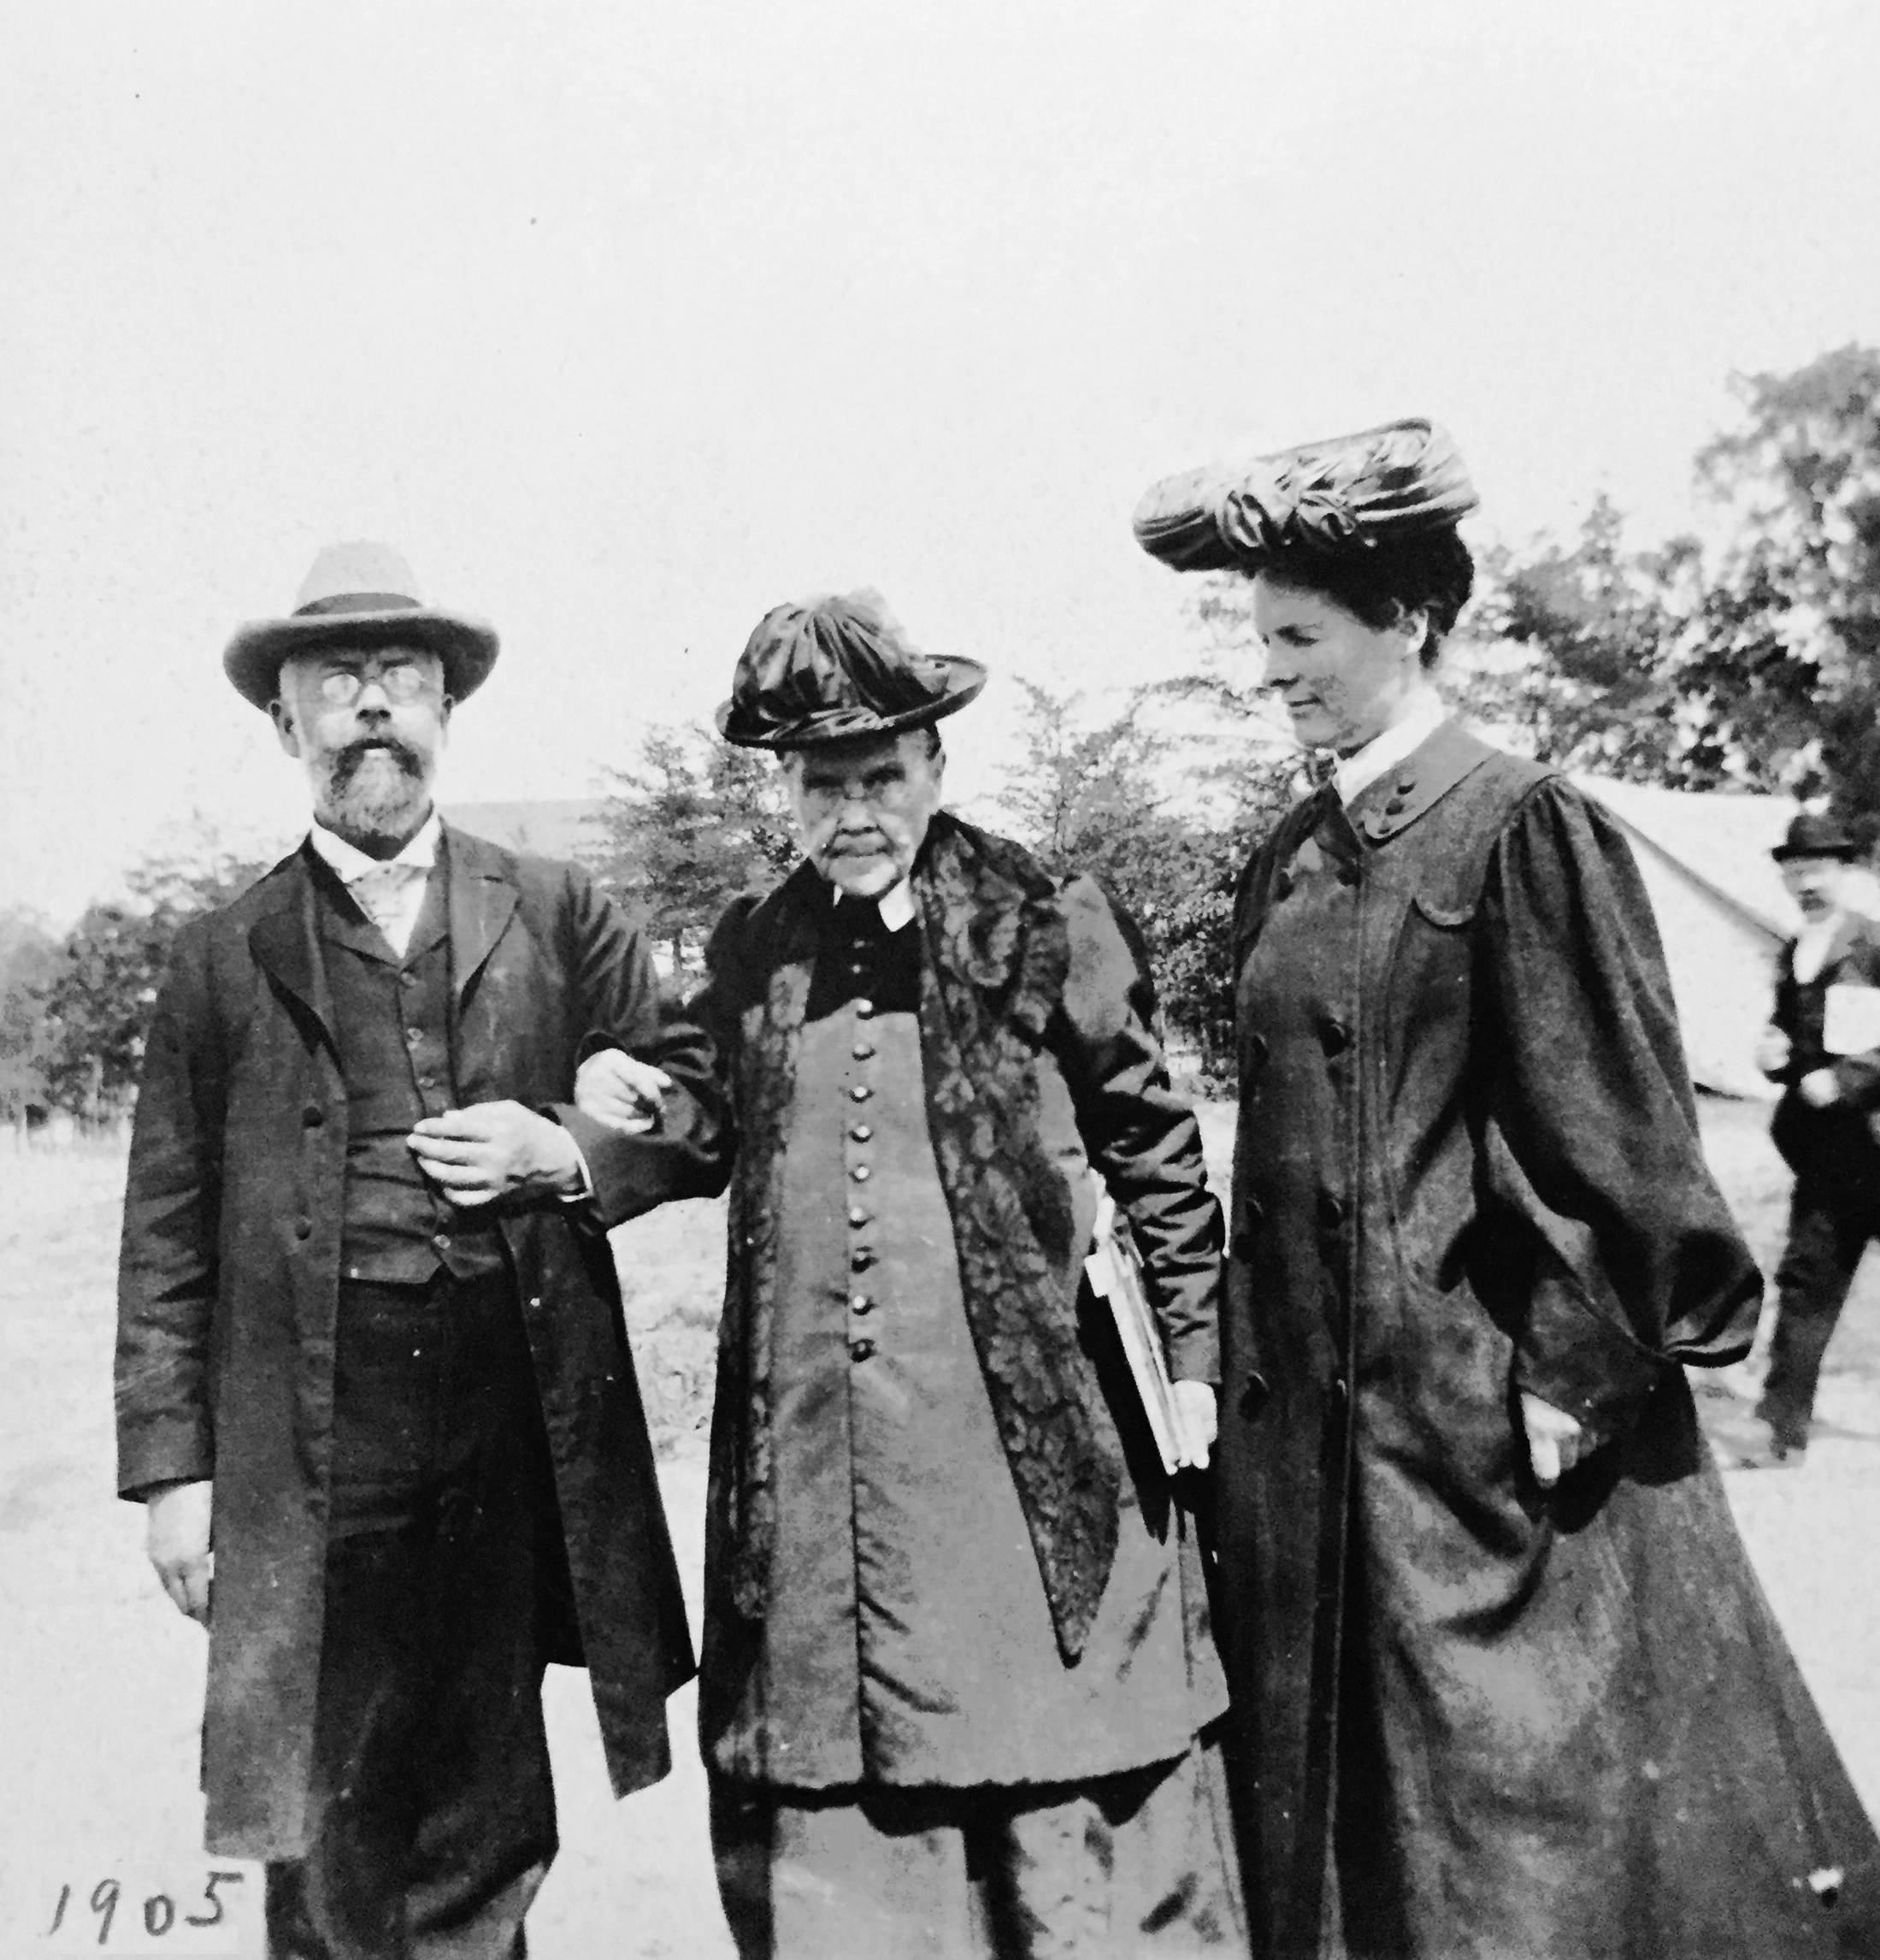
\includegraphics[width=1\linewidth]{images/william-ellen-white-1905.jpg}
    \caption*{William C. White and Ellen G. White, 1905}
    \label{fig:w-e-white}
\end{figure}


\begin{figure}
    \centering
    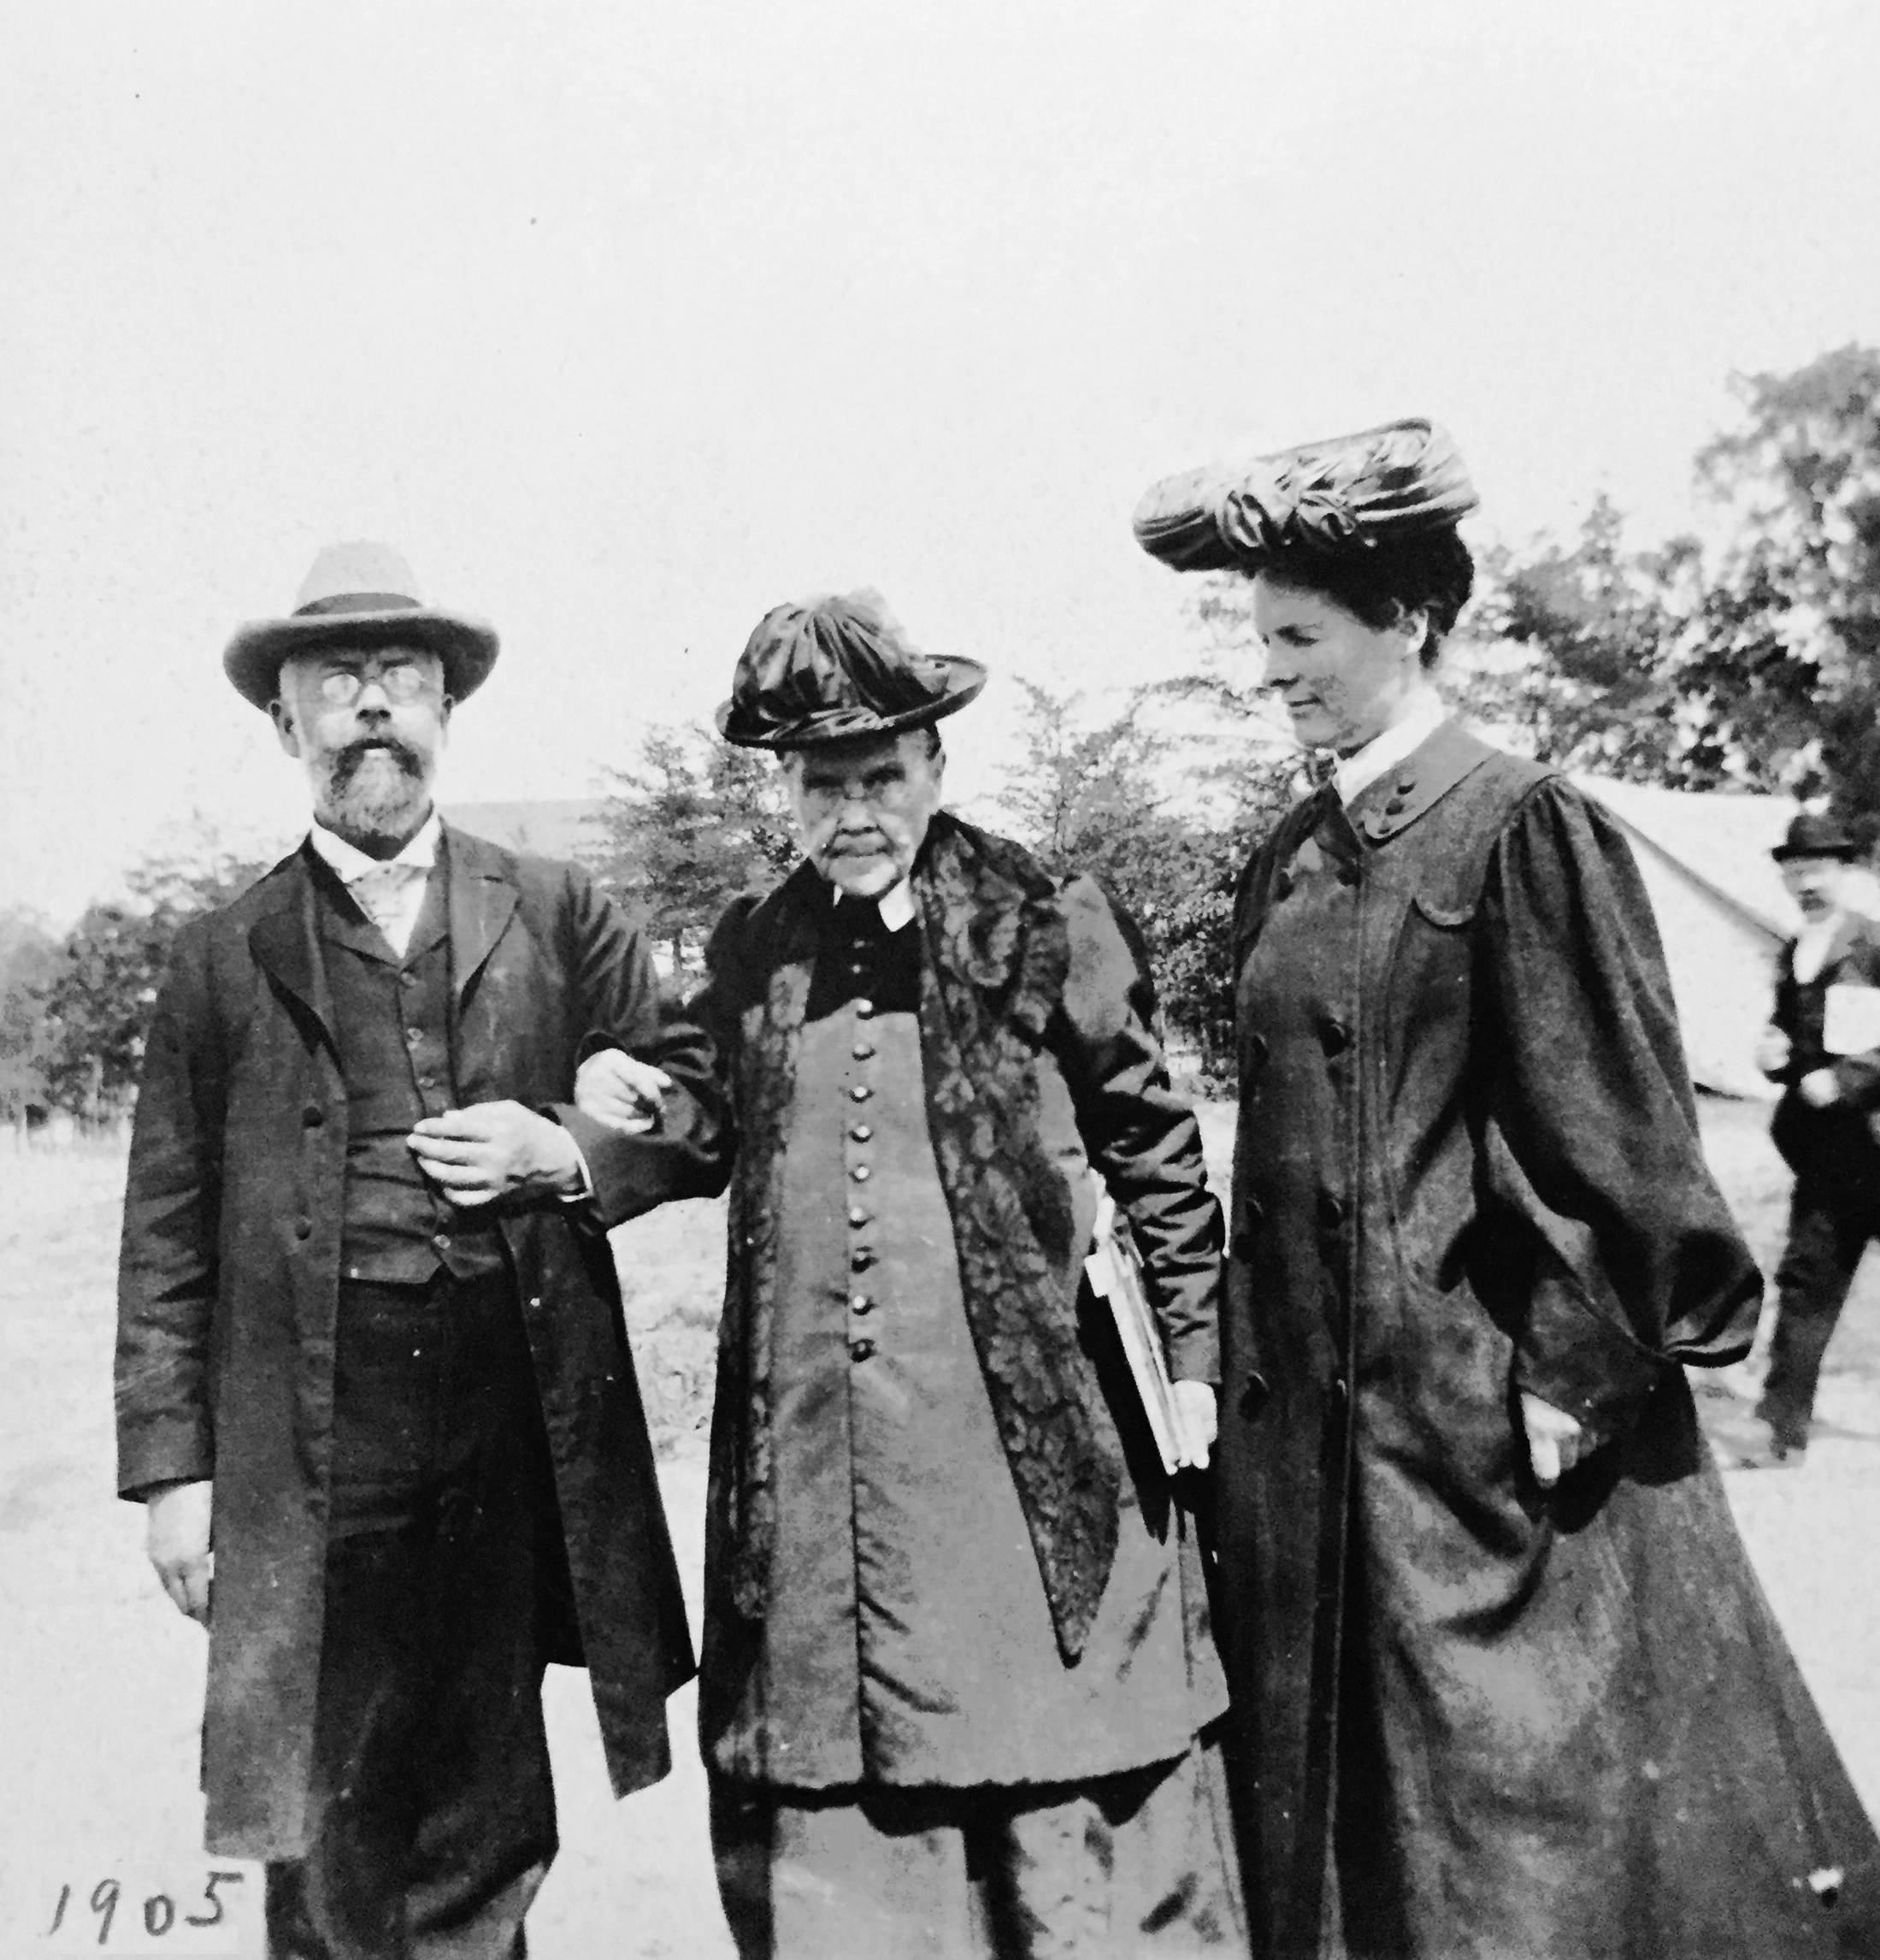
\includegraphics[width=1\linewidth]{images/william-ellen-white-1905.jpg}
    \caption*{ويليام سي. وايت وإلين جي. وايت، 1905}
    \label{fig:w-e-white}
\end{figure}


According to William White, our only hope as Seventh-day Adventists is to adhere to first principles. These principles, as we know, are the \emcap{Fundamental Principles}. Then, he referred to the order in which the enemy is attacking our work. The attack begins with our disunity, then aims to weaken our reverence for the Sabbath and the Sanctuary service, targets our confidence in the Spirit of Prophecy, and finally focuses on confusing our conceptions regarding personal God.


وفقًا لويليام وايت، فإن أملنا الوحيد كأدفنتست سبتيين هو التمسك بالمبادئ الأولى. هذه المبادئ، كما نعلم، هي \emcap{المبادئ الجوهرية}. ثم، أشار إلى الترتيب الذي يهاجم به العدو عملنا. يبدأ الهجوم بانقسامنا، ثم يهدف إلى إضعاف إجلالنا للسبت وخدمة المقدس، ويستهدف ثقتنا في روح النبوة، وأخيرًا يركز على إرباك مفاهيمنا بخصوص الله الشخصي.


Sister White’s response to William White is of a startling nature. She hints to us that the great apostasy is soon to be realized, and that our hope is to adhere to the first principles of our faith—the \emcap{Fundamental Principles}.


إن رد الأخت وايت على ويليام وايت ذو طبيعة مذهلة. فهي تلمح لنا أن الارتداد العظيم سيتحقق قريبًا، وأن أملنا هو التمسك بالمبادئ الأولى لإيماننا - \emcap{المبادئ الجوهرية}.


\egw{Elmshaven, St. Helena, California} \\
\egw{December 4, 1905} \\
\egw{W. C. White} \\
\egw{My dear son - }


\egw{إلمشافن، سانت هيلينا، كاليفورنيا} \\
\egw{4 ديسمبر، 1905} \\
\egw{دبليو. سي. وايت} \\
\egw{ابني العزيز - }


\egw{...}


\egw{...}


\egw{“\textbf{One thing it is certain is soon to be realized—\underline{the great apostasy}, which is developing and increasing and waxing stronger and \underline{will continue} to do so until the Lord shall descend from heaven with a shout. \underline{We are to hold fast the first principles of our denominated faith} and go forward from strength to increased faith. \underline{Ever} we are to keep the faith that has been substantiated by the Holy Spirit of God \underline{from the earlier events of our experience until the present time}.} We need now larger breadth and deeper, more earnest, unwavering faith in the leadings of the Holy Spirit. \textbf{If we needed the manifest proof of the Holy Spirit’s power to confirm truth \underline{in the beginning}, after the passing of the time, \underline{we need today all the evidence in the confirmation of the truth}, when souls are departing from the faith and giving heed to seducing spirits and doctrines of devils.} There must not be any languishing of soul now. If ever there was a period of time when we needed the Holy Spirit’s power in our discourses, in our prayers, in every action proposed, it is now. \textbf{We are not to stop at the first experience, but while we bear \underline{the same message} to the people, \underline{this message is to be strengthened and enlarged}}. \textbf{We are to see and realize the importance of the message made certain by its divine origin}. We are to follow on to know the Lord, that we may know that His going forth is prepared as the morning. Our souls need the quickening from the Source of all power. \textbf{We may be strengthened and confirmed in the past experience \underline{that holds us to the essential points of truth which have made us what we are—Seventh-day Adventists}.}“}[Lt326-1905.2; 1905][https://egwwritings.org/read?panels=p7678.8]


\egw{“\textbf{هناك شيء من المؤكد أنه سيتحقق قريبًا—\underline{الارتداد العظيم}، الذي يتطور ويزداد ويقوى و\underline{سيستمر} في ذلك حتى ينزل الرب من السماء بهتاف. \underline{علينا أن نتمسك بالمبادئ الأولى لإيماننا المسمى} ونمضي قدمًا من قوة إلى إيمان متزايد. \underline{دائمًا} علينا أن نحافظ على الإيمان الذي أكده روح الله القدس \underline{منذ الأحداث المبكرة في تجربتنا حتى الوقت الحاضر}.} نحتاج الآن إلى اتساع أكبر وإيمان أعمق وأكثر جدية وثباتًا في قيادة الروح القدس. \textbf{إذا كنا بحاجة إلى الدليل الظاهر لقوة الروح القدس لتأكيد الحق \underline{في البداية}، بعد مرور الوقت، \underline{نحتاج اليوم كل الأدلة في تأكيد الحق}، عندما تبتعد النفوس عن الإيمان وتصغي إلى أرواح مضللة وتعاليم شياطين.} يجب ألا يكون هناك أي ضعف للنفس الآن. إذا كان هناك وقت نحتاج فيه إلى قوة الروح القدس في خطاباتنا وصلواتنا وفي كل عمل مقترح، فهو الآن. \textbf{لا يجب أن نتوقف عند التجربة الأولى، بل بينما نحمل \underline{نفس الرسالة} للناس، \underline{يجب تقوية هذه الرسالة وتوسيعها}}. \textbf{علينا أن نرى وندرك أهمية الرسالة التي تأكدت بأصلها الإلهي}. علينا أن نتبع لنعرف الرب، حتى نعلم أن خروجه معد كالفجر. تحتاج نفوسنا إلى الإنعاش من مصدر كل قوة. \textbf{يمكن تقويتنا وتأكيدنا في التجربة الماضية \underline{التي تربطنا بالنقاط الأساسية للحق التي جعلتنا ما نحن عليه—أدفنتست سبتيين}.}”}[Lt326-1905.2; 1905][https://egwwritings.org/read?panels=p7678.8]


\egwnogap{\textbf{The past fifty years have not dimmed one jot or principle of our faith as we received the great and wonderful evidences that were made certain to us in 1844, after the passing of the time.} The languishing souls are to be confirmed and quickened according to His Word. And many of the ministers of the gospel and the Lord’s physicians will have their languishing souls quickened according to the Word. \textbf{\underline{Not a word is changed or denied}.} \textbf{That which the Holy Spirit testified to as truth after the passing of the time, in our great disappointment, is \underline{the solid foundation of truth}. Pillars of truth were revealed, and we accepted \underline{the foundation principles} that have made us what we are—Seventh-day Adventists, keeping the commandments of God and having the faith of Jesus.}}[Lt326-1905.3; 1905][https://egwwritings.org/read?panels=p7678.9]


\egwnogap{\textbf{لم تُعتم السنوات الخمسون الماضية ذرة واحدة أو مبدأ من إيماننا كما تلقينا الأدلة العظيمة والرائعة التي تأكدت لنا في عام 1844، بعد مرور الوقت.} يجب تأكيد وإنعاش النفوس الضعيفة وفقًا لكلمته. وسيتم إنعاش نفوس العديد من خدام الإنجيل وأطباء الرب الضعيفة وفقًا للكلمة. \textbf{\underline{لم تتغير أو تُنكر كلمة واحدة}.} \textbf{ما شهد به الروح القدس كحق بعد مرور الوقت، في خيبة أملنا العظيمة، هو \underline{الأساس الصلب للحق}. تم الكشف عن أعمدة الحق، وقبلنا \underline{المبادئ الأساسية} التي جعلتنا ما نحن عليه—أدفنتست سبتيين، نحفظ وصايا الله ولنا إيمان يسوع.}}[Lt326-1905.3; 1905][https://egwwritings.org/read?panels=p7678.9]


This letter is startling because it is an answer to the order of how the enemy is attacking our work. Sister White is well aware of these attacks and she presented the problem in its correct light, also showing us what we shall do to prevent Satan's attacks on us. The enemy wants to \others{confuse our conception regarding a personal God}. This is the very point of great apostasy that \egwinline{is soon to be realized}, and has been \egwinline{developing and increasing and waxing stronger and will continue to do so until the Lord shall descend from heaven with a shout}. This is the apostasy we are experiencing today. What is our hope against this deception and great apostasy? \egwinline{\textbf{\underline{We are to hold fast the first principles of our denominated faith} and go forward from strength to increased faith. \underline{Ever} we are to keep the faith that has been substantiated by the Holy Spirit of God from the earlier events of our experience until the present time.}} \egwinline{...\textbf{\underline{this message is to be strengthened and enlarged}}...} \egwinline{...\textbf{\underline{we need today all the evidence in the confirmation of the truth}}...} \egwinline{\textbf{We may be strengthened and confirmed in the past experience that holds us to the essential points of truth which have made us what we are—Seventh-day Adventists}}. These essential points of truth, which have made us Seventh-day Adventists, are the \emcap{Fundamental Principles}, born in the beginning of our work. In 1905, she wrote, \egwinline{\textbf{The past fifty years have not dimmed one jot or principle of our faith as we received the great and wonderful evidences that were made certain to us in 1844, after the passing of the time.}} \egwinline{\textbf{Not a word is changed or denied.} \textbf{That which the Holy Spirit testified to as truth after the passing of the time, in our great disappointment, is \underline{the solid foundation of truth}. Pillars of truth were revealed, and we accepted \underline{the foundation principles} that have made us what we are—Seventh-day Adventists, keeping the commandments of God and having the faith of Jesus.}}


هذه الرسالة مذهلة لأنها إجابة على ترتيب كيفية مهاجمة العدو لعملنا. الأخت وايت تدرك جيدًا هذه الهجمات وقدمت المشكلة في ضوئها الصحيح، موضحة لنا أيضًا ما يجب أن نفعله لمنع هجمات الشيطان علينا. يريد العدو أن \others{يشوش مفهومنا بخصوص إله شخصي}. هذه هي نقطة الارتداد العظيم التي \egwinline{سيتم تحقيقها قريبًا}، وكانت \egwinline{تتطور وتزداد وتقوى وستستمر في ذلك حتى ينزل الرب من السماء بهتاف}. هذا هو الارتداد الذي نختبره اليوم. ما هو أملنا ضد هذا الخداع والارتداد العظيم؟ \egwinline{\textbf{\underline{علينا أن نتمسك بالمبادئ الأولى لإيماننا المسمى} ونمضي قدمًا من قوة إلى إيمان متزايد. \underline{دائمًا} علينا أن نحافظ على الإيمان الذي أكده روح الله القدس منذ الأحداث المبكرة في تجربتنا حتى الوقت الحاضر.}} \egwinline{...\textbf{\underline{يجب تقوية هذه الرسالة وتوسيعها}}...} \egwinline{...\textbf{\underline{نحتاج اليوم كل الأدلة في تأكيد الحق}}...} \egwinline{\textbf{يمكن تقويتنا وتأكيدنا في التجربة الماضية التي تربطنا بالنقاط الأساسية للحق التي جعلتنا ما نحن عليه—أدفنتست سبتيين}}. هذه النقاط الأساسية للحق، التي جعلتنا أدفنتست سبتيين، هي \emcap{المبادئ الجوهرية}، التي ولدت في بداية عملنا. في عام 1905، كتبت، \egwinline{\textbf{لم تُعتم السنوات الخمسون الماضية ذرة واحدة أو مبدأ من إيماننا كما تلقينا الأدلة العظيمة والرائعة التي تأكدت لنا في عام 1844، بعد مرور الوقت.}} \egwinline{\textbf{\underline{لم تتغير أو تُنكر كلمة واحدة}.} \textbf{ما شهد به الروح القدس كحق بعد مرور الوقت، في خيبة أملنا العظيمة، هو \underline{الأساس الصلب للحق}. تم الكشف عن أعمدة الحق، وقبلنا \underline{المبادئ الأساسية} التي جعلتنا ما نحن عليه—أدفنتست سبتيين، نحفظ وصايا الله ولنا إيمان يسوع.}}


God calls us to be steadfast in the \emcap{Fundamental Principles}, especially over the \others{conception regarding a personal God}. This is the first point of the \emcap{Fundamental Principles}.


يدعونا الله أن نكون ثابتين في \emcap{المبادئ الجوهرية}، خاصة فيما يتعلق \others{بمفهوم إله شخصي}. هذه هي النقطة الأولى من \emcap{المبادئ الجوهرية}.


Sister White foretold that a great apostasy is developing in our church regarding the understanding of the \emcap{personality of God}. The true understanding of the \emcap{personality of God} is presented in the \emcap{Fundamental Principles}. She clearly warned us of Satan’s attack on these principles. She calls us to \egw{\textbf{hold fast the first principles of our denominated faith} and go forward from strength to increased faith}.


تنبأت الأخت وايت بأن ارتدادًا عظيمًا يتطور في كنيستنا فيما يتعلق بفهم \emcap{شخصانية الله}. الفهم الحقيقي \emcap{لشخصانية الله} مقدم في \emcap{المبادئ الجوهرية}. لقد حذرتنا بوضوح من هجوم الشيطان على هذه المبادئ. إنها تدعونا إلى \egw{\textbf{التمسك بالمبادئ الأولى لإيماننا المسمى} والمضي قدمًا من قوة إلى إيمان متزايد}.


\egw{\textbf{“After the passing of the time, God entrusted to His faithful followers the precious \underline{principles of present truth}. These principles were not given to those who had had no part in the giving of the first and second angels’ messages. They were given to the workers who had had a part in the cause from the beginning}.”}[Ms129-1905.5; 1905][https://egwwritings.org/read?panels=p9797.12]


\egw{\textbf{“بعد مرور الوقت، ائتمن الله أتباعه المخلصين على \underline{مبادئ الحق الحاضر} الثمينة. لم تُعط هذه المبادئ لأولئك الذين لم يكن لهم دور في تقديم رسائل الملاك الأول والثاني. بل أُعطيت للعاملين الذين كان لهم دور في القضية منذ البداية}.”}[Ms129-1905.5; 1905][https://egwwritings.org/read?panels=p9797.12]


\egwnogap{\textbf{Those who passed through these experiences are to be as \underline{firm as a rock to the principles} that have made us Seventh-day Adventists}. They are to be workers together with God, binding up the testimony and sealing the law among His disciples. Those who took part in the establishment of our work upon the foundation of Bible truth; \textbf{those who know the waymarks that have pointed out the right path} are to be regarded as workers of the highest value. They can speak from personal experience, regarding the truths entrusted to them. These men are not to permit their faith to be changed to infidelity; they are not to permit the banner of the third angel to be taken from their hands. They are to hold the beginning of their confidence firm unto the end. \textbf{\underline{The Lord has declared that the history of the past shall be rehearsed as we enter upon the closing work}. Every truth that He has given for these last days is to be proclaimed to the world. \underline{Every pillar} that He has established \underline{is to be strengthened}. We cannot now step off the foundation that God has established. We cannot now enter into any new organization; for this would mean apostasy from the truth}.}[Ms129-1905.6; 1905][https://egwwritings.org/read?panels=p9797.13]


\egwnogap{\textbf{أولئك الذين مروا بهذه التجارب يجب أن يكونوا \underline{ثابتين كالصخر على المبادئ} التي جعلتنا أدفنتست سبتيين}. يجب أن يكونوا عاملين مع الله، يربطون الشهادة ويختمون الشريعة بين تلاميذه. أولئك الذين شاركوا في تأسيس عملنا على أساس حق الكتاب المقدس؛ \textbf{أولئك الذين يعرفون المعالم التي أشارت إلى الطريق الصحيح} يجب اعتبارهم عاملين ذوي قيمة عليا. يمكنهم التحدث من تجربة شخصية، بخصوص الحقائق المؤتمنة لهم. هؤلاء الرجال لا يجب أن يسمحوا بتغيير إيمانهم إلى عدم إيمان؛ لا يجب أن يسمحوا بأخذ راية الملاك الثالث من أيديهم. عليهم أن يتمسكوا ببداية ثقتهم ثابتة إلى النهاية. \textbf{\underline{لقد أعلن الرب أن تاريخ الماضي سيُعاد سرده عندما ندخل في العمل الختامي}. كل حق أعطاه لهذه الأيام الأخيرة يجب أن يُعلن للعالم. \underline{كل عمود} أقامه \underline{يجب تقويته}. لا يمكننا الآن الخروج عن الأساس الذي أسسه الله. لا يمكننا الآن الدخول في أي تنظيم جديد؛ لأن هذا سيعني الارتداد عن الحق}.}[Ms129-1905.6; 1905][https://egwwritings.org/read?panels=p9797.13]


Stepping off of the foundation that God has established means entering into new organization; this is apostasy from the truth. Comparing the \emcap{Fundamental Principles} of the past with current trinitarian Fundamental Beliefs, it’s evident we’re in a state of apostasy.  Ellen White prophesied that this apostasy will be \egwinline{\textbf{developing and increasing and waxing stronger and \underline{will continue} to do so until the Lord shall descend from heaven with a shout}}[Lt326-1905.2; 1905][https://egwwritings.org/read?panels=p7678.8].


الخروج عن الأساس الذي أسسه الله يعني الدخول في تنظيم جديد؛ هذا هو الارتداد عن الحق. بمقارنة \emcap{المبادئ الجوهرية} للماضي مع المعتقدات الأساسية الثالوثية الحالية، من الواضح أننا في حالة ارتداد. تنبأت إلين وايت بأن هذا الارتداد سيكون \egwinline{\textbf{يتطور ويزداد ويقوى و\underline{سيستمر} في ذلك حتى ينزل الرب من السماء بهتاف}}[Lt326-1905.2; 1905][https://egwwritings.org/read?panels=p7678.8].


% The great apostasy is soon to be realized

\begin{titledpoem}
    
    \stanza{
        In a letter penned, a crisis foretold, \\
        From Ellen White, a warning bold: \\
        "Adhere to the roots of our Adventist comprehend, \\
        For soon will come apostasy's seed."
    }

    \stanza{
        The pillars strong of our founding year, \\
        Are under siege, as Ellen feared. \\
        To "Meet it!" was her stern command, \\
        To hold the line, to firmly stand.
    }

    \stanza{
        "Keep to the principles," her urgent plea, \\
        From 1844's prophetic decree. \\
        For truth confirmed by the Spirit's flame, \\
        Shall not be denied, nor put to shame.
    }

    \stanza{
        The enemy seeks to divide and sway, \\
        To change our course, to lead astray. \\
        But steadfast hearts must ever cling \\
        To the first truths that made our spirits sing.
    }

    \stanza{
        Hold fast, she wrote, to what we know, \\
        The Fundamental Principles that show \\
        The way to live, the path to trod, \\
        Under the gaze of an unchanging God.
    }

    \stanza{
        For as the world spins toward its close, \\
        The truth of Ellen White still glows— \\
        A beacon strong against the night, \\
        Guiding the faithful in the right.
    }
    
\end{titledpoem}